\documentclass[border=3pt]{standalone}
% Shared preamble for standalone figures (same fonts/colours as the paper).
\usepackage[T1]{fontenc}
\usepackage{lmodern}
\usepackage{amsmath,amssymb}
\usepackage[dvipsnames,svgnames]{xcolor}
\usepackage{tikz}
\usetikzlibrary{arrows.meta,positioning,calc,shapes.geometric,decorations.pathreplacing,shadings}
\usepackage{pgfplots}
\pgfplotsset{compat=1.18}
\usepgfplotslibrary{fillbetween}
\definecolor{pgrey}{HTML}{EEEEEE}
\definecolor{ppink}{HTML}{F8D7DA}
\definecolor{ppeach}{HTML}{FDE5C8}
\definecolor{porange}{HTML}{FBC78D}
\definecolor{pgreen}{HTML}{D4F7D4}
\definecolor{ppurple}{HTML}{EFE3F7}
\definecolor{pblue}{HTML}{DCE8F7}
\definecolor{dgreen}{HTML}{2E8B2E}
\definecolor{dpink}{HTML}{C2185B}
\definecolor{dorange}{HTML}{E07B00}
\definecolor{dblue}{HTML}{1F4E9E}
\definecolor{dpurple}{HTML}{7B3FA0}
\definecolor{gold}{HTML}{E0A800}
\tikzset{
  blk/.style={draw=black!70,rounded corners=2pt,minimum height=0.8cm,minimum width=1.9cm,
              align=center,font=\sffamily\footnotesize,inner sep=3pt},
  arr/.style={-{Stealth[length=2.2mm]},thick,black!75},
  darr/.style={-{Stealth[length=2mm]},dashed,thick},
  lbl/.style={font=\itshape\scriptsize},
}

\begin{document}
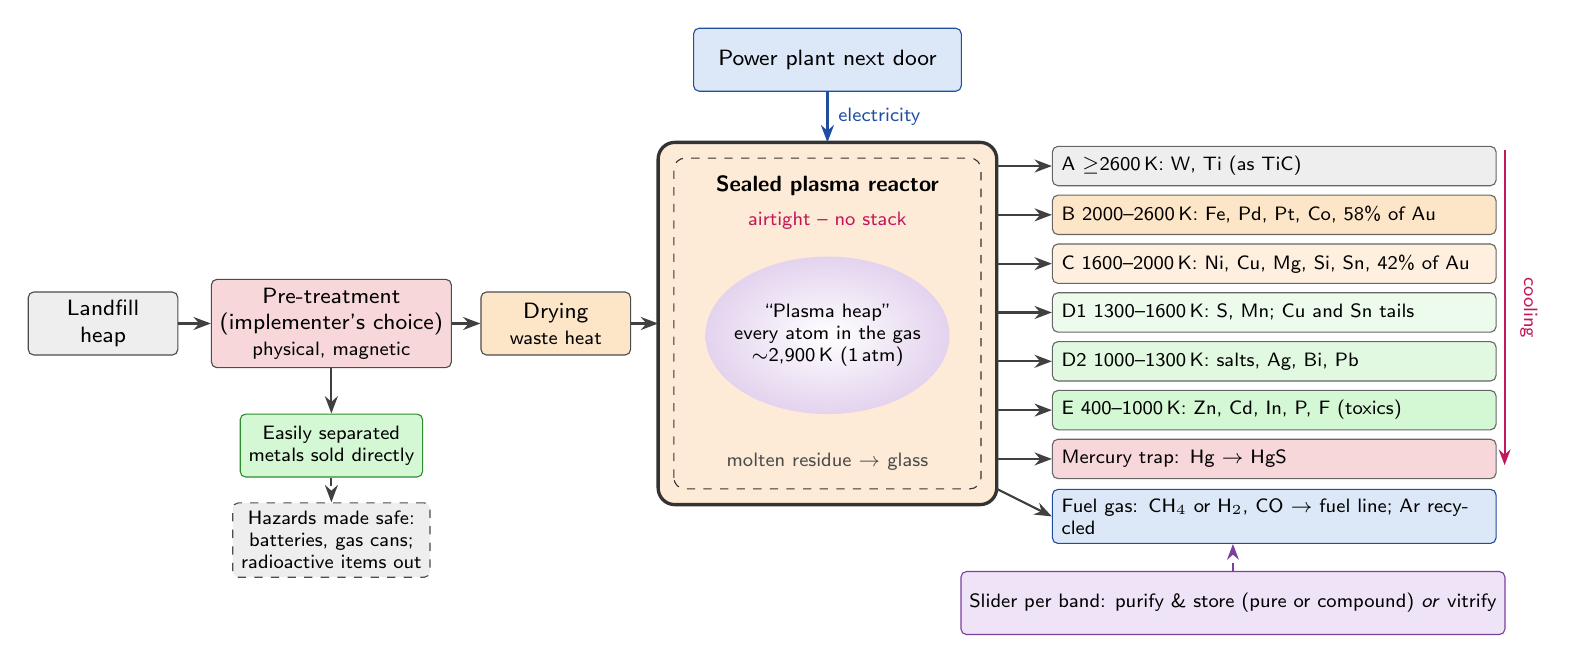
\begin{tikzpicture}
% power plant next door
\node[blk,fill=pblue,draw=dblue,minimum width=3.4cm] (power) at (8.75,3.35) {Power plant next door};
% front end
\node[blk,fill=pgrey] (heap) at (-0.45,0) {Landfill\\heap};
\node[blk,fill=ppink] (split) at (2.45,0) {Pre-treatment\\(implementer's choice)\\\scriptsize physical, magnetic};
\node[blk,fill=ppeach] (dry) at (5.3,0) {Drying\\\scriptsize waste heat};
\node[blk,fill=pgreen,draw=dgreen,font=\sffamily\scriptsize] (steel) at (2.45,-1.55) {Easily separated\\metals sold directly};
\node[blk,fill=pgrey,font=\sffamily\scriptsize,dashed] (haz) at (2.45,-2.75) {Hazards made safe:\\batteries, gas cans;\\radioactive items out};
% sealed reactor
\draw[very thick,black!80,rounded corners=6pt,fill=porange!35] (6.6,-2.3) rectangle (10.9,2.3);
\draw[black!80,rounded corners=4pt,dashed] (6.8,-2.1) rectangle (10.7,2.1);
\node[font=\sffamily\footnotesize\bfseries,align=center] at (8.75,1.75) {Sealed plasma reactor};
\node[font=\sffamily\scriptsize,align=center,text=dpink] at (8.75,1.3) {airtight -- no stack};
\shade[inner color=white,outer color=ppurple!90!dpurple] (8.75,-0.15) ellipse (1.55 and 1.0);
\node[font=\sffamily\scriptsize,align=center] at (8.75,-0.15) {``Plasma heap''\\every atom in the gas\\$\sim$2,900\,K (1\,atm)};
\node[font=\sffamily\scriptsize,text=black!70] at (8.75,-1.75) {molten residue $\to$ glass};
% ladder
\foreach \y/\t/\c [count=\k] in {
  2.0/{A $\ge$2600\,K: W, Ti (as TiC)}/pgrey,
  1.38/{B 2000--2600\,K: Fe, Pd, Pt, Co, 58\% of Au}/ppeach,
  0.76/{C 1600--2000\,K: Ni, Cu, Mg, Si, Sn, 42\% of Au}/ppeach!60,
  0.14/{D1 1300--1600\,K: S, Mn; Cu and Sn tails}/pgreen!45,
  -0.48/{D2 1000--1300\,K: salts, Ag, Bi, Pb}/pgreen!70,
  -1.10/{E 400--1000\,K: Zn, Cd, In, P, F (toxics)}/pgreen,
  -1.72/{Mercury trap: Hg $\to$ HgS}/ppink}{
  \node[draw=black!60,fill=\c,rounded corners=2pt,font=\sffamily\scriptsize,anchor=west,minimum height=0.5cm,text width=5.4cm] (b\k) at (11.6,\y) {\t};
  \draw[arr] (10.9,\y) -- (b\k.west);}
\node[draw=dblue,fill=pblue,rounded corners=2pt,font=\sffamily\scriptsize,anchor=west,minimum height=0.62cm,text width=5.4cm] (gas) at (11.6,-2.45) {Fuel gas: CH$_4$ or H$_2$, CO $\to$ fuel line; Ar recycled};
\draw[arr] (10.9,-2.1) -- (gas.west);
\draw[-{Stealth[length=2mm]},thick,dpink] (17.35,2.2) -- node[right,font=\sffamily\scriptsize,rotate=-90,anchor=south,yshift=2pt]{cooling} (17.35,-1.8);
% slider
\node[blk,fill=ppurple,draw=dpurple,minimum width=6.8cm,font=\sffamily\scriptsize] (slider) at (13.9,-3.55) {Slider per band: purify \& store (pure or compound) \emph{or} vitrify};
% flows
\draw[arr] (heap) -- (split);
\draw[arr] (split) -- (dry);
\draw[arr] (dry) -- (6.6,0);
\draw[arr] (split) -- (steel);
\draw[arr,dashed] (steel) -- (haz);
\draw[-{Stealth[length=2.2mm]},very thick,dblue] (power) -- node[right,font=\sffamily\scriptsize]{electricity} (8.75,2.3);
\draw[darr,dpurple] (slider.north) -- (13.9,-2.8);
\end{tikzpicture}
\end{document}
